O método do Gradiente Conjugado nada mais é do que um ajuste sobre o método do Gradiente descrito na seção \ref{sec:descida_max}. As mudanças de direção abruptas, conforme ilustrado na figura \ref{fig:stegradeszigzag}, são suavizadas com a adição do coeficiente de inércia $\beta$, que conserva uma fração da direção anterior. Assim, a direção de avanço toma a seguinte forma:
	\begin{equation}
	d^{k+1} = -g(x^{k+1}) + \beta_k d^k
	\end{equation}
A Lei de Iteração é a mesma do método do Gradiente:
		\begin{align}
			x^{k+1} &= x^k + \alpha_k d^k \\
			\tilde{f}(\alpha) &= f(x^k + \alpha d^k)
		\end{align}
A função $\tilde{f}(\alpha)$ é minimizada utilizando a razão áurea.\\
Já o coeficiente $\beta$ é uma relação entre o gradiente atual e o anterior.\\
		Segundo \textit{Polak-Rebière}:
		\begin{equation}
			\beta_k = \frac{||g^{k+1}|| - [g^+1]^T g^k}{||g^k||}
		\end{equation}
Com essa suavização das direções de avanço, é esperado que esse método convirja com menos iterações do que o método do Gradiente. 

Depois de construído o algoritmo, foram testadas quatro funções para efeitos de comparação:

\begin{itemize}
	\item $ f_1(x,y) = x^2 + y^2$
	\item $ f_2(x,y) = -e^{-x^2 -y^2}$
	\item $ f_3(x,y) = cos(\frac{xy}{5})+sin(\frac{xy}{5}) $
	\item $ f_4(x,y) = |x+y| $
\end{itemize}

\begin{figure}[H]
	\begin{center}
		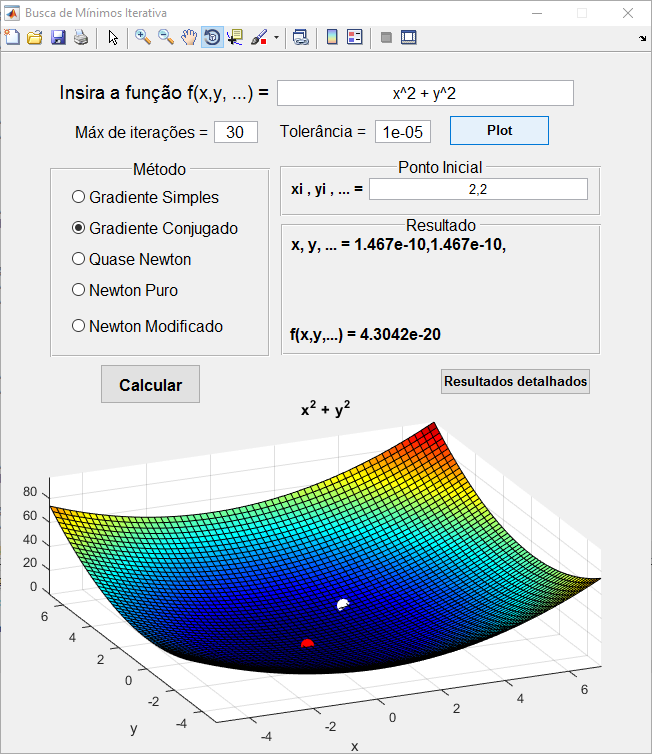
\includegraphics[width=12cm]{../gradiente_conjugado/f1_gui}   
		\caption{Janela de inicialização de $ f_1(x,y) $}
		\label{fig:gradiente_conjugado_f1_gui}
	\end{center}
\end{figure}

\begin{figure}[H]
	\begin{center}
		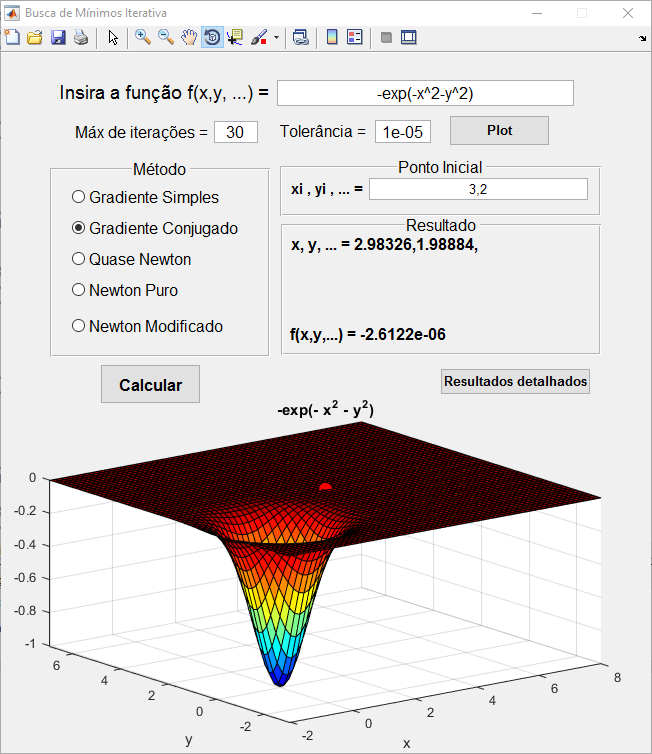
\includegraphics[width=12cm]{../gradiente_conjugado/f2_gui}   
		\caption{Janela de inicialização de $ f_2(x,y) $}
		\label{fig:gradiente_conjugado_f2_gui}
	\end{center}
\end{figure}

\begin{figure}[H]
	\begin{center}
		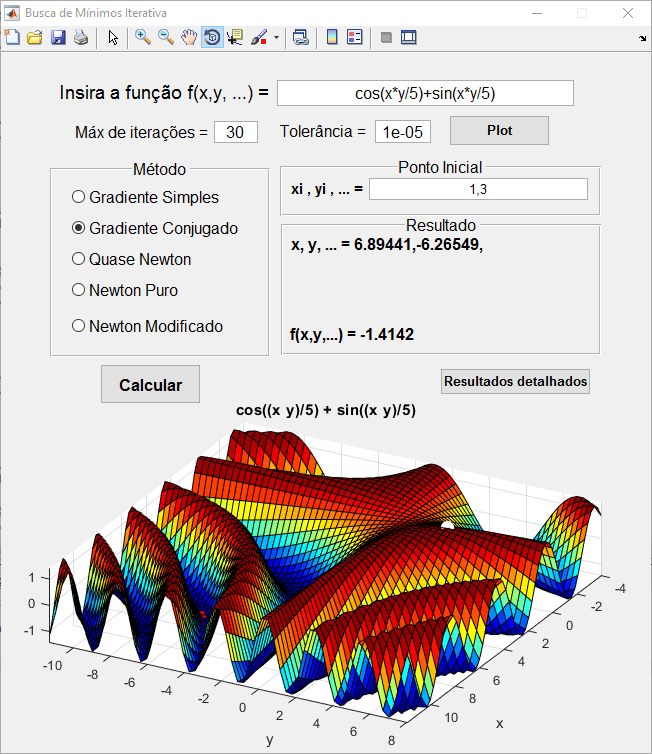
\includegraphics[width=12cm]{../gradiente_conjugado/f3_gui}   
		\caption{Janela de inicialização de $ f_3(x,y) $}
		\label{fig:gradiente_conjugado_f3_gui}
	\end{center}
\end{figure}


\begin{figure}[H]
	\begin{center}
		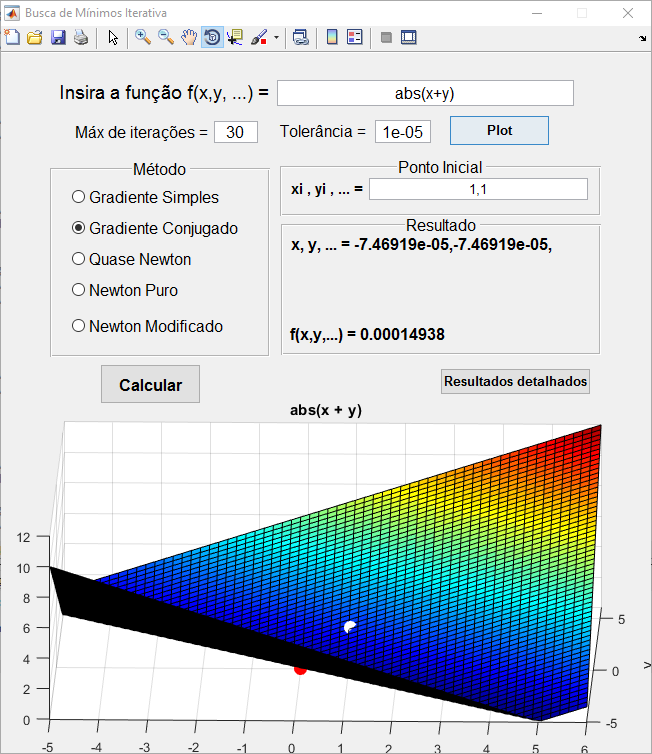
\includegraphics[width=12cm]{../gradiente_conjugado/f4_gui}   
		\caption{Janela de inicialização de $ f_4(x,y) $}
		\label{fig:gradiente_conjugado_f4_gui}
	\end{center}
\end{figure}
